% !TeX spellcheck = en_US
\documentclass[a4paper,12pt,titlepage, twoside]{report} 

\usepackage[latin1]{inputenc}
\usepackage{amssymb}
\usepackage{amsthm}
\usepackage[fleqn]{amsmath}
\usepackage[dvipsnames]{xcolor}
\usepackage{relsize}
\usepackage{paralist}
\usepackage{graphicx}
\usepackage[super]{nth}
\usepackage{relsize}
\usepackage[linesnumbered, ruled]{algorithm2e}
\usepackage[section]{placeins}
\usepackage{pdfpages}
\usepackage{biblatex}
\addbibresource{cites.bib}



\newcommand{\suaca}{\textbf{SUACA}}
\newcommand{\iaca}{\textbf{IACA}}
\newcommand{\microop}{$\mu$op}
\newcommand{\microops}{$\mu$ops}

%\usepackage{bnf}
%\usepackage{epsf}
\usepackage{appendix}

%\usepackage[a4paper]{geometry}
%\geometry{left=3cm,right=3cm,top=23mm,bottom=25mm,head=14.5pt}

\usepackage{phdthesis}
\setlength{\headheight}{15pt}
\usepackage{listings}
\lstdefinelanguage{myLang}
{
    % list of keywords
    morekeywords={
        movl,
        byte,
        mov,
        cmp,
        jne,
        add,
        jmp,
        else,
        end
    },
    sensitive=false, % keywords are not case-sensitive
    morecomment=[l]{//}, % l is for line comment
}
\lstset{showspaces=false,showstringspaces=false,breaklines=true,breakindent=0pt,
        prebreak={},
        postbreak=\mbox{{ }},
    escapeinside={(*@}{@*)},
    language=C,
    basicstyle=\ttfamily,
    keywordstyle=\color{blue}\ttfamily,
    stringstyle=\color{red}\ttfamily,
    commentstyle=\color{green}\ttfamily,
    morecomment=[l][\color{magenta}]{\#}
}
\usepackage{makeidx}          % wir wollen auch einen Index
\usepackage{hyperref}
%\renewcommand*{\figureautorefname}{figure}
\usepackage{tikz}
\usetikzlibrary{matrix,backgrounds, shapes, arrows.meta}
\tikzset{mynode/.style={draw, ellipse, thick, line width = 2pt}}
\usepackage{tkz-graph}
\SetUpEdge[lw         = 1.5pt,
           style={->},
           color      = black,
           labelcolor = white,
           labeltext  = red,
           labelstyle = {draw,text=black}]

\tikzset{bright/.style = {bend right=23, ->}}
\tikzset{bleft/.style = {bend left=23, ->}}

\definecolor{light-gray}{gray}{0.95}
\usepackage{mdframed}
\usepackage{pgfplots}
\usepackage{changepage}
\usepackage{fancyvrb}
\usepackage{wrapfig}
\usepackage{lipsum}
\parindent0pt
\newtheorem{theorem}{Theorem}
\newtheorem{definition}{Definition}

\begin{document}
\setlength{\oddsidemargin}{\dimexpr (\paperwidth-\textwidth)/2 - 1in\relax}
\setlength{\evensidemargin}{\oddsidemargin}

\begin{titlepage}
\setlength{\topmargin}{0cm}

\begin{changetext}{2cm}{0cm}{0cm}{0cm}{0cm}
   
  

%\let\footnotesize\small \let\footnoterule\relax
\begin{center}

%\hbox{}
%\vfill

\includegraphics[width=4cm]{eule}
\vskip 1cm
Saarland University\\
Faculty of Natural Sciences and Technology I\\
Department of Computer Science\\[2ex]
\setlength{\textheight}{2cm}
\vskip 1cm
{\large \bfseries Bachelor Thesis}

\vskip .75cm
{\huge\bfseries SUACA \par}
{A tool for performance analysis of machine programs \par}

\vskip 1.5cm

submitted by\\
\vskip .25cm
{\large Hendrik Meerkamp}
\\

\vskip 1cm

submitted\\
\vskip .25cm
\today

\vskip 1.5cm

Supervisor\\
\vskip .25cm
Prof. Dr. Sebastian Hack\\
\vskip .5cm
Advisor \\
\vskip .25cm
Andreas Abel\\
\vskip .5cm
Reviewers\\
\vskip .25cm
Prof. Dr. Sebastian Hack\\
Prof. Dr. Jan Reineke
\end{center}
\end{changetext}
\vfill
\end{titlepage}

\newpage
\thispagestyle{empty}
\mbox{}

\includepdf[pages=2]{deckblatt_BA_MA_Dipl_eid_bibo_engl.pdf}

\newpage
\thispagestyle{empty}
\mbox{}

\begin{abstract}
Abstract
\end{abstract}


\newpage
\thispagestyle{empty}
\mbox{}

\setcounter{page}{0}
\tableofcontents 


%----------------------------------------------------------------------------------------
%	Introduction
%----------------------------------------------------------------------------------------

\chapter{Introduction}

\section{Motivation}

Knowing your machine is a major advantage when trying to optimize high-performance scientific code. \iaca\ \cite{iaca} is a tool by Intel to analyze \emph{X86} machine code with respect to a specific microarchitecture. However, it has some drawbacks that often times prevent it from being useful in practice. The main reason is that doesn't support the newest processors. \iaca\ $3.0$, which released in late 2017, supports the \nth{4} (Haswell) to the \nth{6} (Skylake) generation of Intel microarchitectures. Skylake was released in 2015. \iaca\ $2.3$ additionally supports the \nth{2} (Sandy Bridge) and the \nth{3} (Ivy Bridge) generation. So at the time of writing \iaca\ is about three years behind and further development remains unclear.\\
The second complication is that \iaca\ is closed source. Its user guide \cite{userguide} is the only documentation it has which provides little to no information about how it actually computes its output. As a result a user will often find himself wondering how its output fits the analyzed program.\\
In this work we present \suaca\ (Saarland University Architecture Code Analyzer), an open source alternative. It uses measurements provided by \cite{Andreas} which are parsed during runtime. This way a user doesn't rely on a software update of the tool as he can simply perform the measurements on his own, should we not already support his microarchitecture. Note that this is only possible with Intel architectures so far. At the time of writing \suaca\ supports all Intel microarchitectures from the \nth{1} (Nehalem) to the \nth{8} (Coffee Lake) generation, except for the server variant of Skylake.

\newpage
\section{Scope of work}

Like mentioned before we will present a tool that is able to analyze given \emph{X86} assembler code in respect to a specific microarchitecture. Just like \iaca\ our tool is able to find byte markers inside a compiled file and analyze the code in between. Those markers can be inserted in two different ways: inserting them by hand in the assembler code or use the \emph{iacaMarks.h} header in your \emph{C} code. First take a look at the assembly variant:

\begin{mdframed}[backgroundcolor=light-gray, roundcorner=10pt,leftmargin=1, rightmargin=1, innerleftmargin=15, innertopmargin=1,innerbottommargin=1, outerlinewidth=1, linecolor=light-gray]
\begin{lstlisting}[language={myLang}]
 movl $111, %ebx
.byte 0x64, 0x67, 0x90

    //Some code here
    
 movl $222, %ebx
.byte 0x64, 0x67, 0x90
\end{lstlisting}
\end{mdframed}

When using a loop \emph{C} code one can easily insert the markers defined in the \emph{iacaMarks.h} header like this:

\begin{mdframed}[backgroundcolor=light-gray, roundcorner=10pt,leftmargin=1, rightmargin=1, innerleftmargin=15, innertopmargin=1,innerbottommargin=1, outerlinewidth=1, linecolor=light-gray]
\begin{lstlisting}
#include "iacaMarks.h"

int main(void) {

    while (condition) {
        (*@\textcolor{Green}{IACA\_START}  @*)
        //Some code here
    }
    (*@\textcolor{Green}{IACA\_END}  @*)

    return 0;
}
\end{lstlisting}
\end{mdframed}

In both cases a user has to compile his code and run \suaca\ on the compiled file. We are using Intel's \emph{X86 Encoder Decoder
} library \cite{xed} to disassemble said file, which allows us to support files of the \emph{ELF}, \emph{PECOFF} and \emph{MACHO} format.\\
After disassembling \suaca\ will perform a dependency analysis on the instructions and parse the measurement file. After that is done it will perform a simulation of the code. It won't consider the actual effect of the instructions, only their latencies, dependencies and port usage. For several reasons, which we will discuss in the following, our simulation will compute an estimate of the code's performance, not total numbers.\\
\suaca\ is able to perform several kinds of analyses which we will discuss in \autoref{chap:functionality}. In \autoref{chap:algorithms} we will then explain in detail how the most important parts of the simulation and the dependency analyzes are done.


\section{Intel's microarchitectures}


\begin{wrapfigure}[25]{l}{0.6\textwidth}
    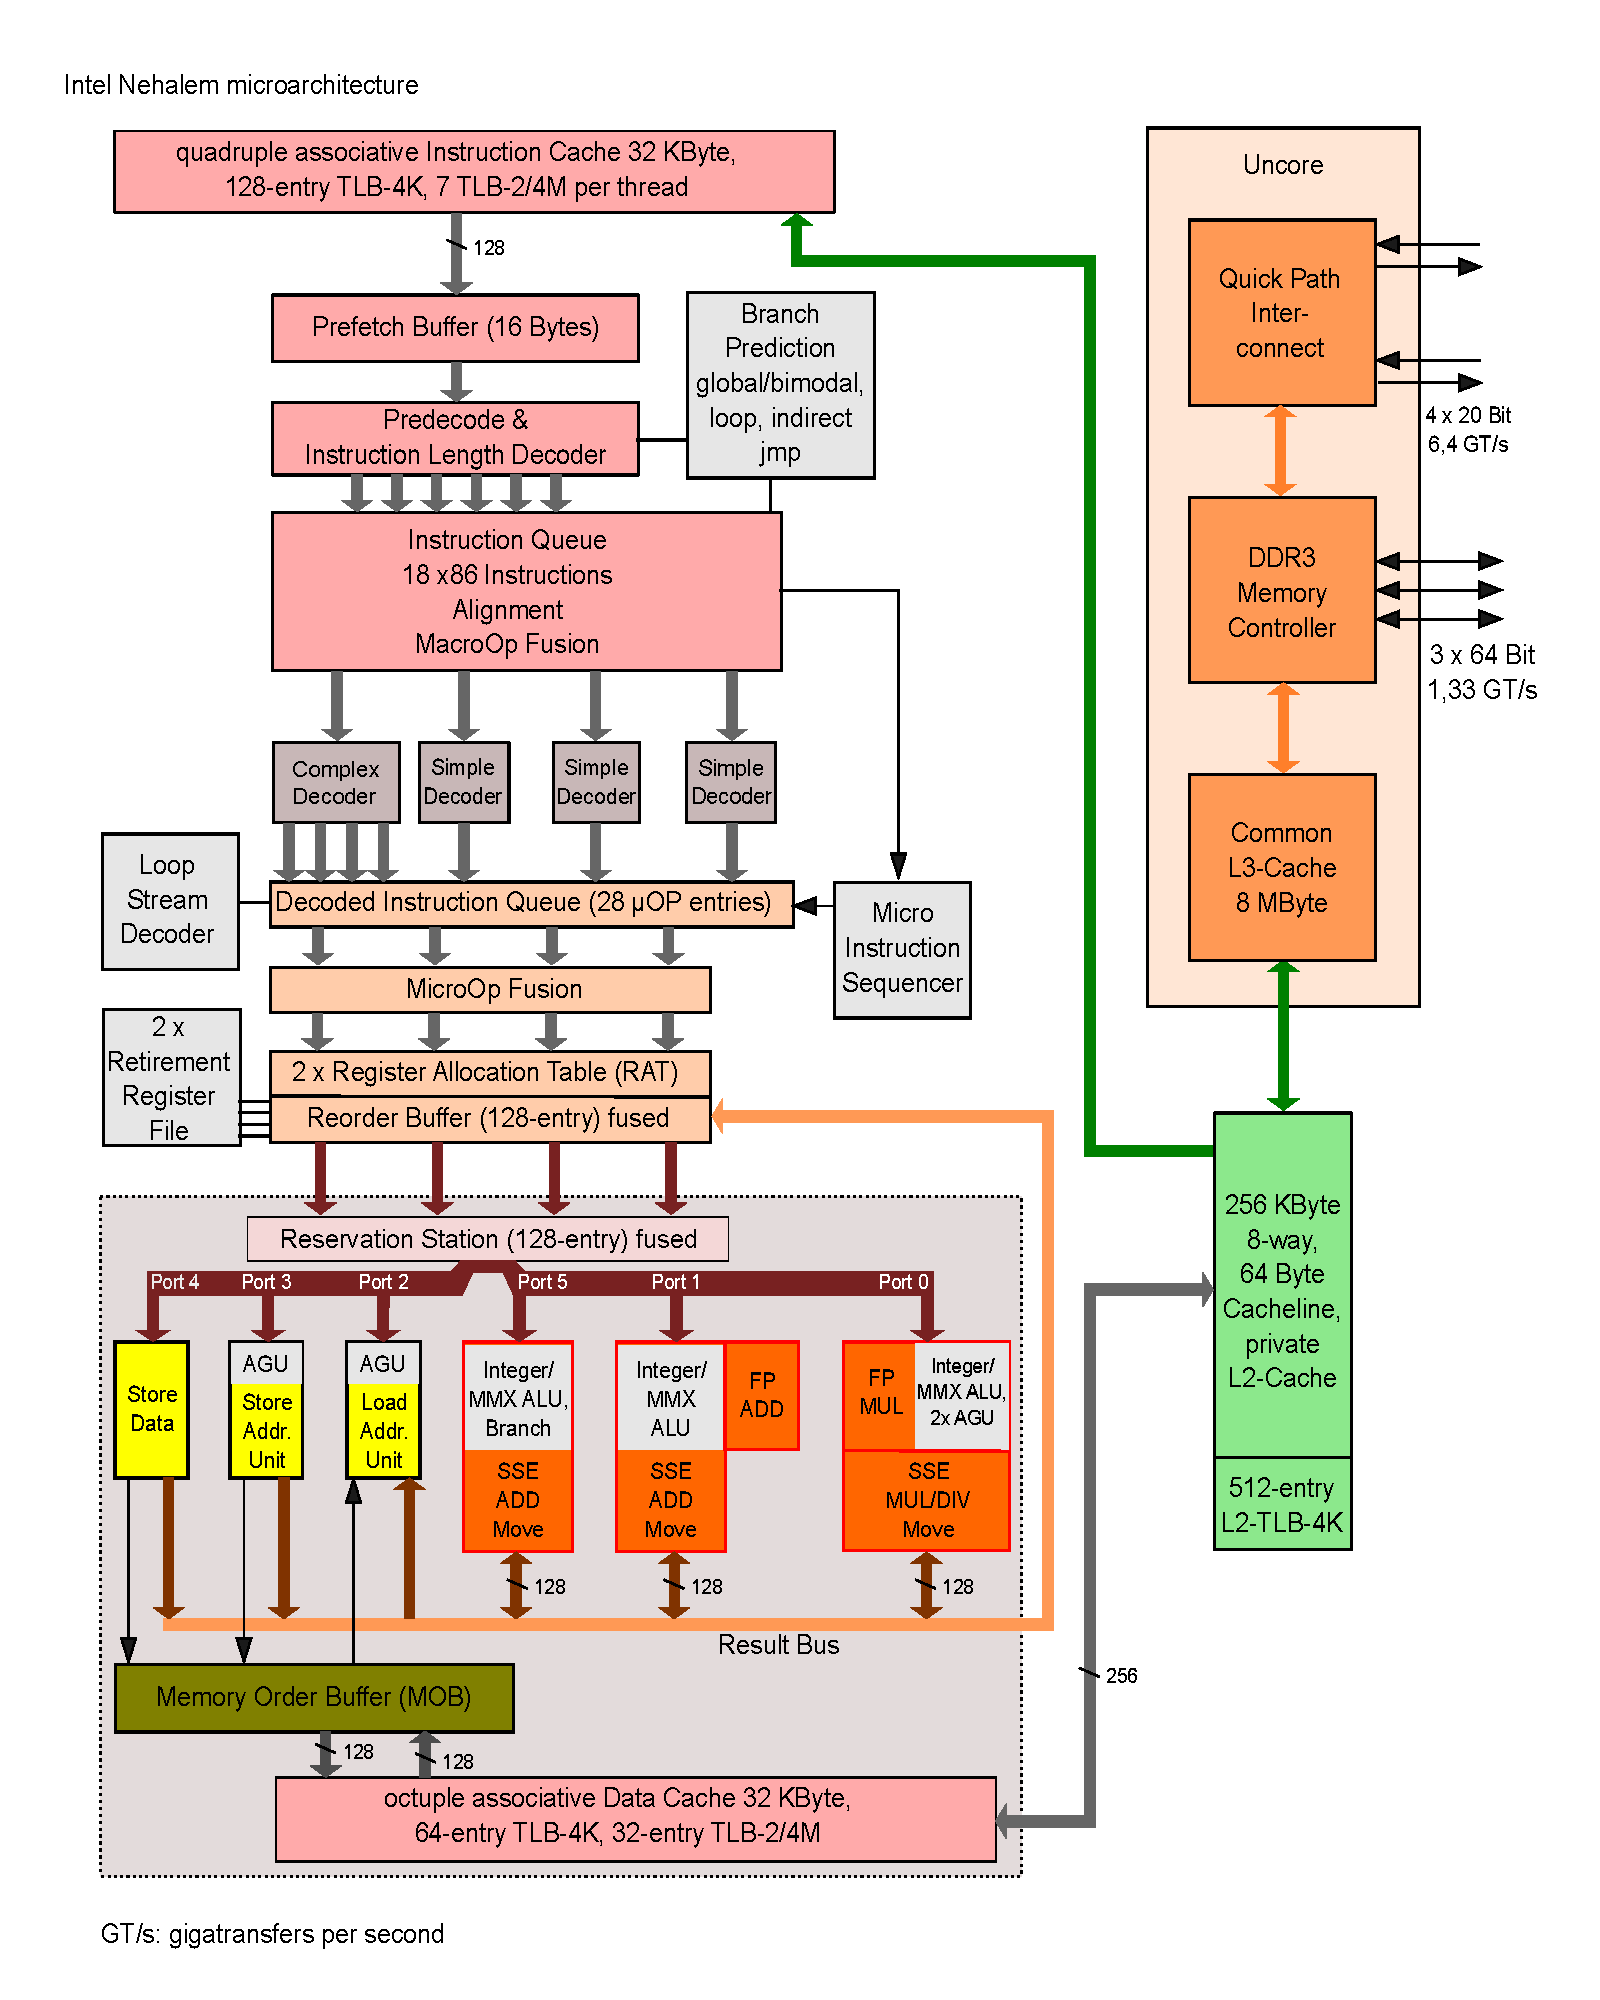
\includegraphics[width=0.6\textwidth]{Intel_Nehalem_arch}
    \caption{Intel Nehalem architecture \cite{nehalem}}
    \label{fig:NHMfull}
\end{wrapfigure}


In order to understand some of our computations one also needs some basic knowledge about Intel's microarchitectures. They use the \emph{X86} instruction set. However, they don't execute those instructions directly. They will translate them into a sequence of so called \microops, which can then be executed. Unfortunately there is little to no documentation about those \microops, neither about the functionality of an individual one nor about their interaction with each other. From our measurements we can conclude that each microarchitecture has its own \microops which makes it even harder to find reliable information.\\ \autoref{fig:NHMfull} shows a sketch of the Nehalem architecture. We can see the decoders which are responsible for the translation of the \microops, but most of this sketch is not of particular interest for us. In our simulation we will consider most of this as the ``front end'' which will only be simulated by the number of \microops\ it produces each cycle. Our main interest lies in the gray dotted rectangle shown by \autoref{fig:NHMdetail}.\\
This figure shows the reservation station (or scheduler). It is responsible for the distribution of the \microops\ over the ports. As mentioned before, each cycle a certain amount of those will be loaded into the reservation station.


\begin{wrapfigure}[15]{r}{0.6\textwidth}
    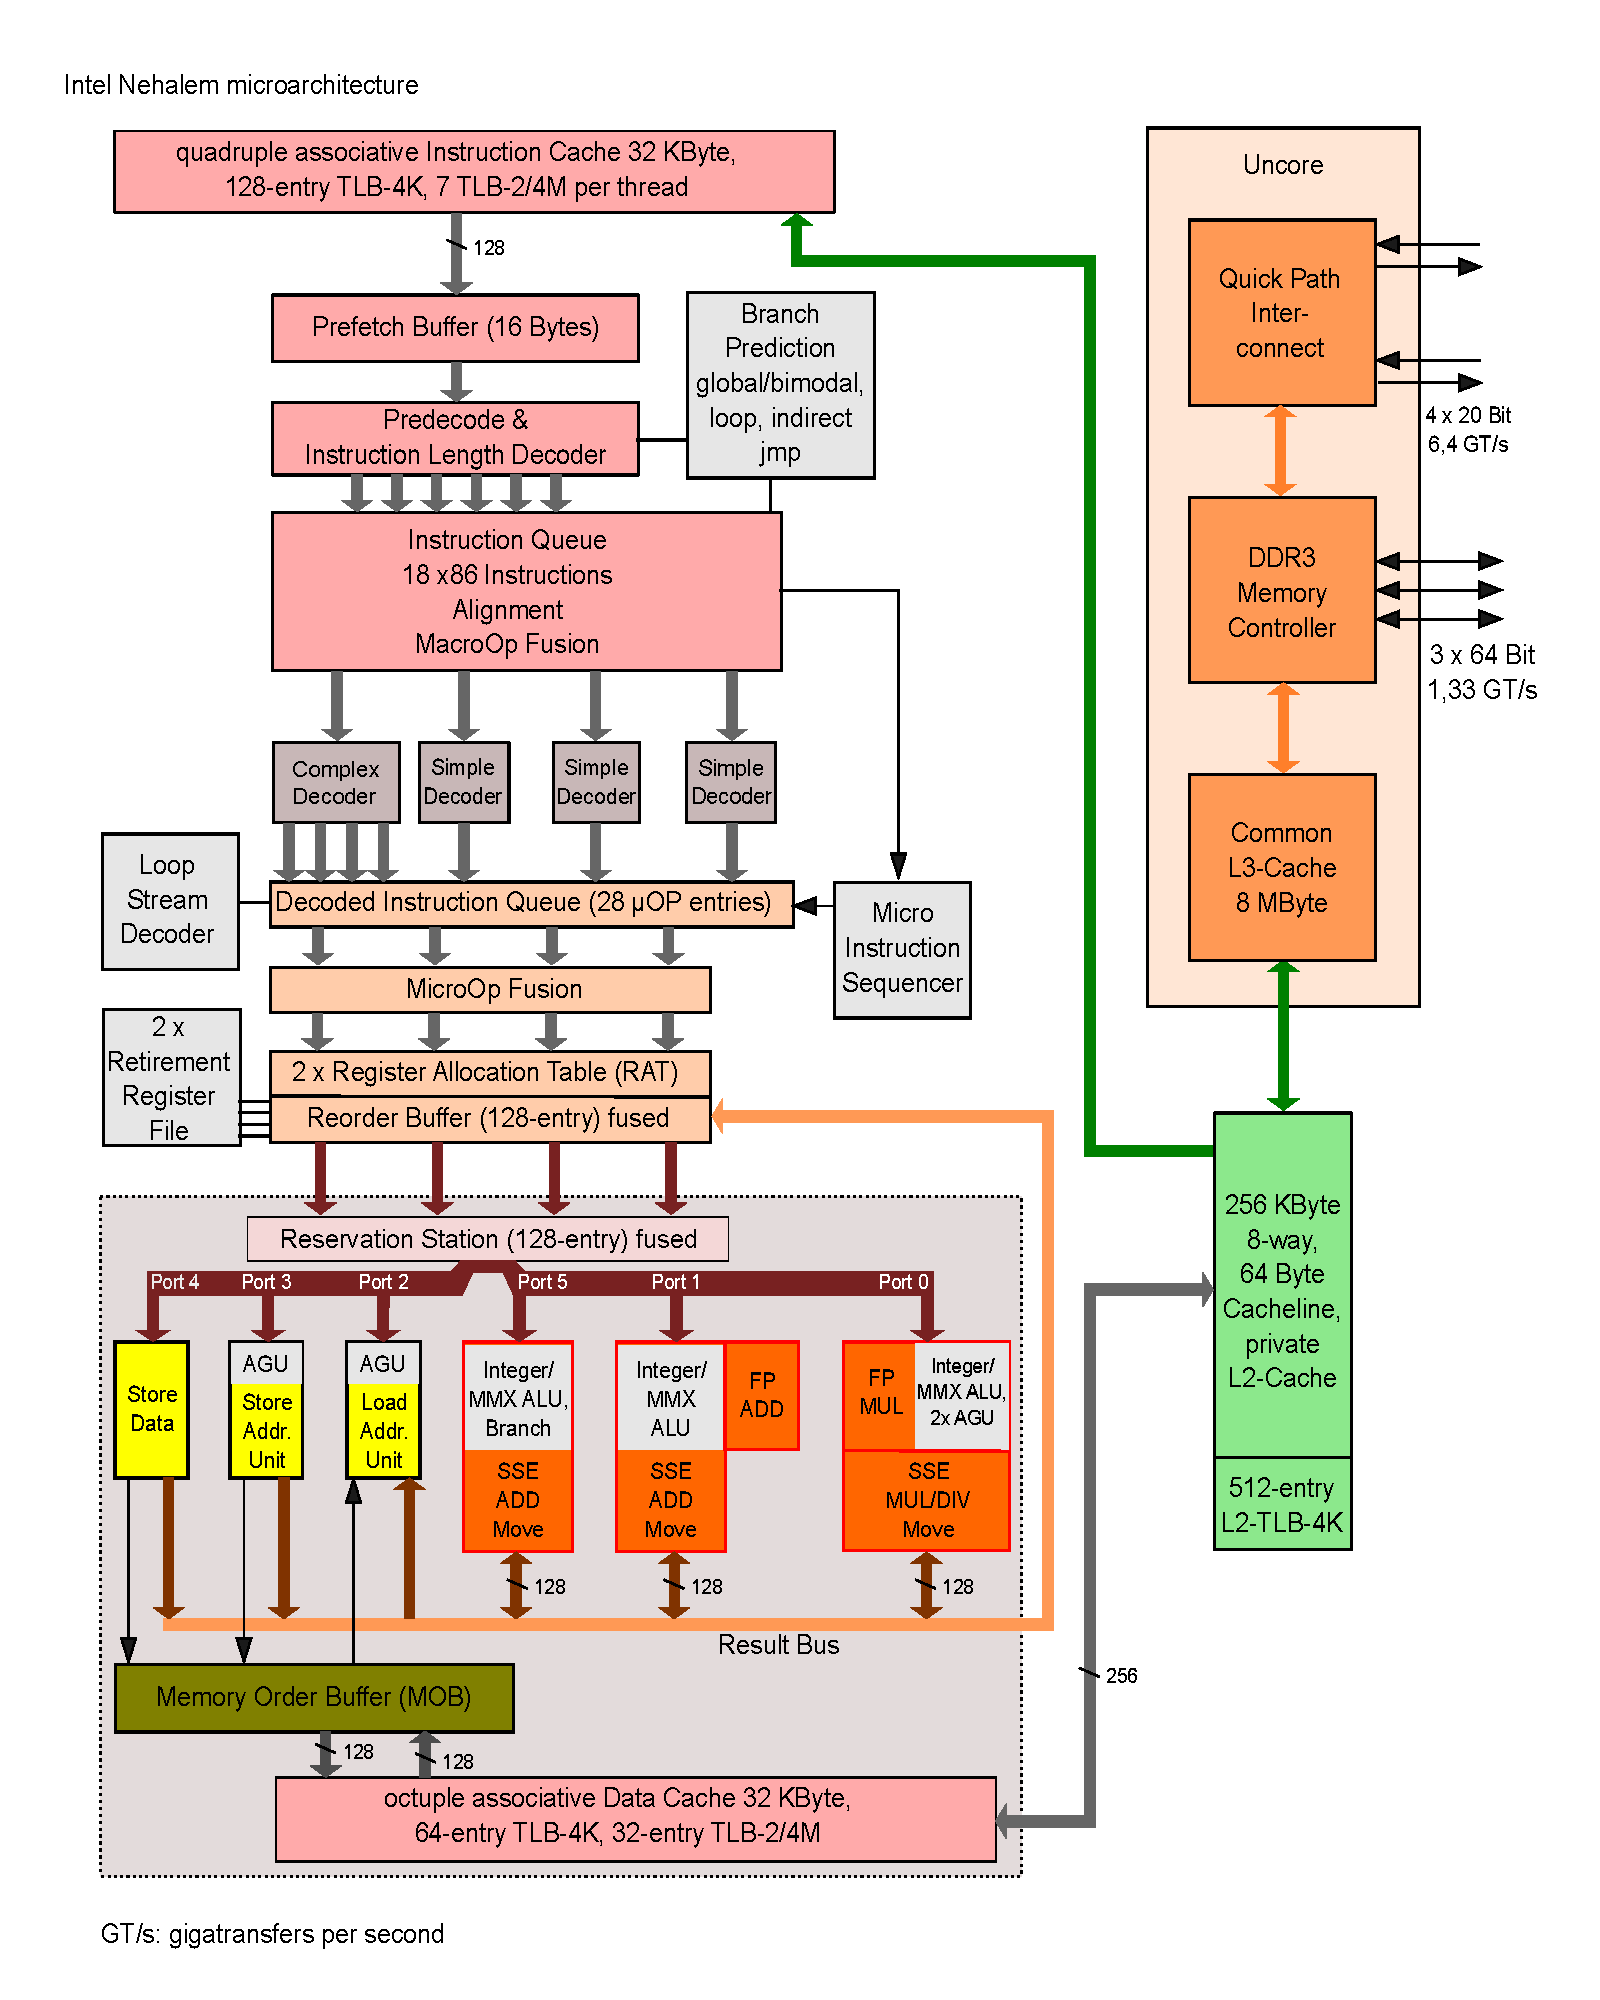
\includegraphics[clip, trim=0.5cm 2cm 9.78cm 20cm,width=0.6\textwidth]{Intel_Nehalem_arch}
    \caption{Detailed view}
    \label{fig:NHMdetail}
\end{wrapfigure}

 How many depends on the architecture, in the case of Nehalem it's $4$. The capacity also depends on the specific architecture. The important property we can observe from this figure are the ports. Each port can be seen as a pipeline that a \microop\ can run through in order to be executed. On the ports themselves lie the actual execution units of the processor like the \emph{ALU}, \emph{MULTIPLEXER} and so on. Every port can hold a single \microop\ per cycle and they support pipelining. So they will be free again in the next cycle. The only exception from this is the \emph{DIVIDER} unit which is slow at executing and can block a port for multiple cycles.

\section{Measurements}
\label{sec:measurements}

As mentioned before a crucial part of \suaca's functionality are the measurements provided by \cite{Andreas}. Consider this snippet from the XML-measurement-file file:


\begin{lstlisting}[language=XML, basicstyle=\ttfamily\scriptsize, breaklines=false]
<instruction ... iform="ADD_LOCK_MEMv_GPRv" ...>
    <operand idx="2" type="reg" ...>RAX,RCX,RDX,RBX,...</operand>
    <operand idx="3" type="flag" ...>OF</operand>
    <operand idx="4" type="flag" ...>SF</operand>
    ...
    <architecture name="NHM">
        <measurement port15="2" port2="1" port3="1" port4="1" total_uops="5">
            <latency cycles="19" ... targetOp="3"/>
            <latency cycles="19" ... targetOp="4">
            ...
        <\measurement>
    </architecture>
<\instruction>
\end{lstlisting}

We dotted out some unnecessary or redundant information. As we can see in the first line this is the information for the instruction with the \emph{iform} ``ADD\_LOCK\_MEMv\_GPR''. \emph{iform} is an enum from the XED Library (\cite{xed}) that is used to identify instructions. We can extract the following information from our snippet:

\begin{itemize}
    \item One of the \emph{RAX, RCX, RDX, \dots} registers is an operand and they have the id $2$. We only need the mapping of $id \rightarrow register$ here as the xed library will tell us which operands are actually used in the analyzed programs. Similarly the flags also have their ids. The flags are the single bits of the \emph{RFLAGS} register in \emph{X86}.
    \item We have some measurements for the intel nahelem architecture.
    \item When simulating NHM the instruction consists of $5$ \microops. Two of which can use ports $1$ and $5$. One each can use port $2$, port $3$ and port $4$.
    \item It will take $19$ cycles to compute the result for the operand with id $3$. Most instructions have several latency items, depending on the number and kind of operands. In our case there is no information for operand $2$ as the instruction won't write to those registers. However, the latency for the operand with id $4$ is also $19$ cycles. Some instructions actually produce their results in a specific order. It might be that one operand is available after $3$ cycles and another one after $5$, so an instruction that only needs the first of those operands has to wait $3$ cycles whereas another one that needs the second operand has to wait $5$. \suaca\ can simulate this behavior as it knows which operand is causing the dependency. When simulating the whole instruction \suaca\ takes the maximum of those values.
\end{itemize}








%----------------------------------------------------------------------------------------
%	Functionality of SUACA
%----------------------------------------------------------------------------------------

\chapter{Functionality of SUACA}
\label{chap:functionality}
In this chapter we're going to explain and show the full functionality of \suaca. First we will take a look at the command line interface and then see an example run of each available option.

\section{The command line interface}
The CLI of works as follows:\\
\[
suaca\ [option]\ path\_to\_file
\]
Where $[option]$ is one or several of the following:
\begin{itemize}
    \item $-cfg$ will print the control flow graph into a file called $controlflow.dot$. The format will be graphviz readable.
    \item $-dg$ will print the dependencygraph into a file called $dependency.dot$. The format will also be graphviz readable.
    \item $-p$ triggers the ``performance mode''.
    \item $-b$ triggers the branch analysis.
    \item ${--}arch\ x$ will consider $x$ as the underlaying micro-architecture of the analysis. At the time of writing the available options are NHM, SNB, IVB, HSW, BDW, SKL, CFL and KBL. The default value is SNB.
    \item ${--}loop\ x$ will trigger the loop analysis. The default value of $x$ is $1$.
    \item ${--}detail\ x$ will print detailed information about line $x$.
    \item ${--}setup\ x\ y$ sets the default values.
    \item ${--}print-default$ prints the defaults.
\end{itemize}

We will use the following example code to show the effects of each of those options:

\begin{mdframed}[backgroundcolor=light-gray, roundcorner=10pt,leftmargin=1, rightmargin=1, innerleftmargin=15, innertopmargin=1,innerbottommargin=1, outerlinewidth=1, linecolor=light-gray]
\begin{lstlisting}[language={myLang}, basicstyle=\small]
   mov rax, 1
   cmp rcx, 0
   jne else
   add rbx, rax
   jmp end
else:
   add rbx, rax
end:
   add rbx, rbx
\end{lstlisting}
\end{mdframed}

\section{Plain analysis}
\label{sec:plain}
Running \suaca\ without any of the options above will result in the following output:

\begin{mdframed}[backgroundcolor=light-gray, roundcorner=10pt,leftmargin=1, rightmargin=1, innerleftmargin=15, innertopmargin=15,innerbottommargin=15, outerlinewidth=1, linecolor=light-gray]
\begin{center}
\begin{BVerbatim}[fontsize=\tiny]
Block throughput: 3.00 cycles
Block throughput with perfect front end: 3.00 cycles
Block throughput with non-blocking ports: 3.00 cycles
Block throughput with perfect front end and non-blocking ports: 3.00 cycles
Microops per cycle: 2.33

Analysis for architecture: SNB

 Line ||   Num   ||   had   || caused  ||                    Used Ports
      ||   Uops  || to wait || to wait ||   0   ||   1   ||   2   ||   3   ||   4   ||   5   ||
------------------------------------------------------------------------------------------------
  0   ||    1    ||         ||   1.0   ||  1.0  ||       ||       ||       ||       ||       || mov rax, 0x1
  1   ||    1    ||         ||   1.0   ||       ||  1.0  ||       ||       ||       ||       || cmp rcx, 0x0
  2   ||    1    ||   1.0   ||   1.0   ||       ||       ||       ||       ||       ||  1.0  || jnz 0x7
  3   ||    1    ||   1.0   ||   1.0   ||  1.0  ||       ||       ||       ||       ||       || add rbx, rax
  4   ||    1    ||   1.0   ||         ||       ||       ||       ||       ||       ||  1.0  || jmp 0x5
  5   ||    1    ||         ||   1.0   ||       ||  1.0  ||       ||       ||       ||       || add rbx, rax
  6   ||    1    ||   1.0   ||         ||  1.0  ||       ||       ||       ||       ||       || add rbx, rbx
\end{BVerbatim}
\end{center}
\end{mdframed}


At the beginning one will notice the following values:
\begin{itemize}
    \item \textbf{Block throughput} is the number of cycles needed to execute the program once ($\frac{Total\ number\ of\ cycles}{Number\ of\ iterations}$).
    \item \textbf{Block throughput with perfect front end} can be used to see if the front end of the processor was the bottleneck of the execution. To compute this value \suaca\ will perform a full analysis of the program. However, it will assume that $number\ of\ \mu ops\ loaded\ per\ cycle = capacity\ of\ reservation\ station$. If the runtime experiences a speedup we can conclude that the front end was indeed the bottleneck.
    \item \textbf{Block throughput with non-blocking ports} is computed similarly. It will perform a full analysis, but every port can be used arbitrarily. Should the runtime improve we can conclude that one of the ports has to be the bottleneck.
    \item \textbf{Block throughput with perfect front end and non-blocking ports} is a combination of the two above. In some corner cases it might be possible that both front end and ports are responsible for a decreased runtime. This can happen if every loaded instruction is directly computed (front end bottleneck), but if the front end was faster there wouldn't be another port to run the additionally loaded instructions on. In this case none of the first values would differ from the normal \textbf{Block throughput} although they are actually both part of the bottleneck.
\end{itemize}


In the table we can observe the following columns:
\begin{itemize}
    \item The \textbf{had to wait} column describes the number a cycles the instruction experienced a delay from either blocked ports or a value dependence. 
    \item The \textbf{caused to wait} column describes the number of cycles the instruction caused a delay similar to the \textbf{had to wait} value. However, it won't track transitive dependencies. So consider a program that has a dependency chain of $A \rightarrow B \rightarrow C$ (where $A$, $B$ and $C$ are instructions of your program) and $A$ is not fully computed. $A$ will cause $B$ to be delayed, resulting in an increased \textbf{caused to wait} value of $A$. $B$ will then cause $C$ to be delayed, resulting in an increased \textbf{caused to wait} value of $B$.
    \item The \textbf{Used Ports} columns describe how many \microops\ were assigned to this port. If possible \suaca\ will always assign a \microop\ to the port that has been used the least during the analysis (out of the ports that this particular \microop\ is able to use) in order to achieve an even distribution of the ports. A detailed description of how those are computed can be found in ~\autoref{sec:chooseport}.
\end{itemize}

A closer look at the concrete values of this particular run reveals that the sum of the \textbf{caused to wait} column is $5$ whereas the \textbf{had to wait} column only sums up to $4$. This is due to the fact that both line $3$ and $5$ are responsible for the delay of line $6$ because of the dependence via the $rbx$ register. The exact dependencies can be found in ~\autoref{fig:wloop}. The same behavior arises when an instruction can't be executed because all ports are blocked. When $3$ different instructions $A, B$ and $C$ block the ports another instruction $D$ would like to use the \textbf{caused to wait} values of $A, B$ and $C$ are increased while only one \textbf{had to wait} value ($D$'s) will increase.




\section{Loop analysis}
\label{sec:loop}
As we mentioned above the major use case of \iaca\ is analyzing an innermost loop. While \iaca\ will therefore always assume a loop (and ``choose'' the number of iterations) \suaca\ will give the user the option to run the simulation in a loop with the $--loop\ x$ flag. First consider the \suaca\ run of our example program with the flag $--loop\ 200$ set:

\begin{mdframed}[backgroundcolor=light-gray, roundcorner=10pt,leftmargin=1, rightmargin=1, innerleftmargin=15, innertopmargin=15,innerbottommargin=15, outerlinewidth=1, linecolor=light-gray]
\begin{center}
\begin{BVerbatim}[fontsize=\tiny]
Block throughput: 2.34 cycles
Block throughput with perfect front end: 2.34 cycles
Block throughput with non-blocking ports: 2.00 cycles
Block throughput with perfect front end and non-blocking ports: 2.00 cycles
Microops per cycle: 2.99

Analysis for architecture: SNB

 Line  ||   Num   ||   had   || caused  ||            Used Ports
       ||   Uops  || to wait || to wait ||   0   ||   1   ||   2   ||   3   ||   4   ||   5   ||
------------------------------------------------------------------------------------------------
   0   ||    1    ||  15.1   ||  43.2   ||  0.0  ||  1.0  ||       ||       ||       ||       || mov rax, 0x1
   1   ||    1    ||  15.8   ||  32.3   ||  0.3  ||  0.3  ||       ||       ||       ||  0.3  || cmp rcx, 0x0
   2   ||    1    ||  16.5   ||  20.8   ||       ||       ||       ||       ||       ||  1.0  || jnz 0x7
   3   ||    1    ||  15.5   ||  28.9   ||  0.7  ||  0.3  ||       ||       ||       ||       || add rbx, rax
   4   ||    1    ||  16.8   ||  20.4   ||       ||       ||       ||       ||       ||  1.0  || jmp 0x5
   5   ||    1    ||  15.2   ||  28.9   ||  0.3  ||  0.7  ||       ||       ||       ||       || add rbx, rax
   6   ||    1    ||  15.8   ||  43.9   ||  1.0  ||       ||       ||       ||       ||       || add rbx, rbx
\end{BVerbatim}
\end{center}
\end{mdframed}

When running the simulation in a loop the following values will become averages per iteration:

\begin{itemize}
    \item had to wait
    \item caused to wait
    \item used ports
\end{itemize} 

More specifically they will be computed with $\frac{total\ value}{number\ of\ iterations}$.\\
We can observe that line $0$ has used port $0$ $0.0$ times. This just means that this instruction has used port $0$, but to a very little amount and if we remember our \hyperref[sec:plain]{first run}, which didn't use the $loop$ option, we can see that line $0$ in fact uses port $0$ at least once.\\
When looking at the block throughput values we can see that our example program runs quite significantly faster with non-blocking ports. And this makes sense as only ports $0, 1$ and $5$ can be used by the instructions we're using. The two jump instructions are the biggest offender as they can exclusively use port $5$.\\
We can also see that the values of the \textbf{caused to wait} column are a lot higher than those of the \textbf{had to wait} column. This is due to the fact, that several lines can be the cause of another line to be delayed as we already explained in ~\autoref{sec:plain}.

\section{Control flow graph}
The control flow graph is mainly used to compute the correct dependency graph. The $CFG$ of our example program can be seen in ~\autoref{fig:cfg}. The red edge only appears if the analysis runs in a loop as it represents the ``back jump'' to the start of the program that won't appear in a single iteration.

\begin{figure}
    \centering
    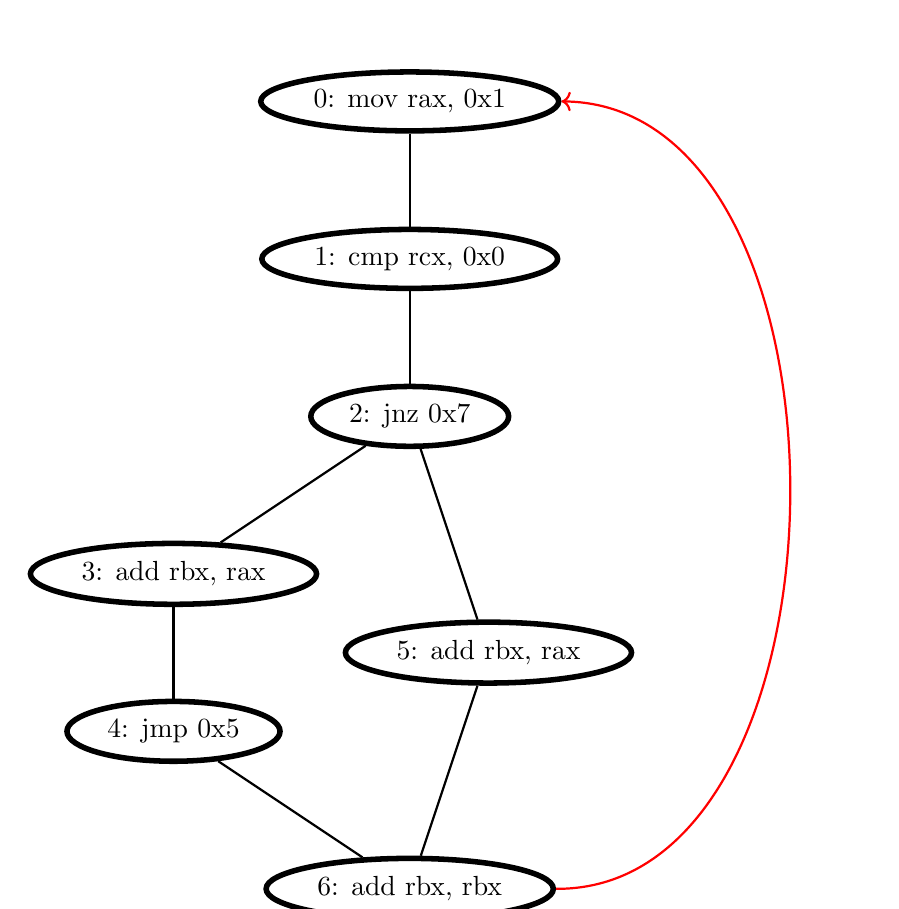
\begin{tikzpicture}
    \node[mynode] (A) at (0, 0)     {0: mov rax, 0x1};	
    \node[mynode] (B) at (0, -2)    {1: cmp rcx, 0x0};
    \node[mynode] (C) at (0, -4)    {2: jnz 0x7};
    \node[mynode] (D) at (-3, -6)   {3: add rbx, rax};
    \node[mynode] (E) at (-3, -8)   {4: jmp 0x5};
    \node[mynode] (F) at (1, -7)    {5: add rbx, rax};
    \node[mynode] (G) at (0, -10)   {6: add rbx, rbx};
    
    
    
    \Edges[](A,B);
    \Edges[](B,C);
    \Edges[](C,D);
    \Edges[](C,F);
    \Edges[](D,E);
    \Edges[](E,G);
    \Edges[](F,G);
    \Edges[style={->, bend right = 90}, color=red](G,A);
    
    \end{tikzpicture}
    \caption{Control flow graph}
    \label{fig:cfg}
\end{figure}

\FloatBarrier

\section{Dependencygraph}
The dependency graph describes all register dependencies that occur in the program. An edge from node $A$ to node $B$ means that the instruction represented by $B$ depends on the instruction represented by $A$. \suaca\ will only track read-after-write dependencies. Whenever an instruction uses a memory address \suaca\ will try to extract all used registers. It won't keep track of the stack as this would often times require runtime specific information. The detailed algorithm that is used to generate this graph can be seen at ~\autoref{sec:depanalysis}. First consider this graph that will be generated in the ``single loop case'' in \autoref{fig:woloop}.\\


\begin{figure}
\centering
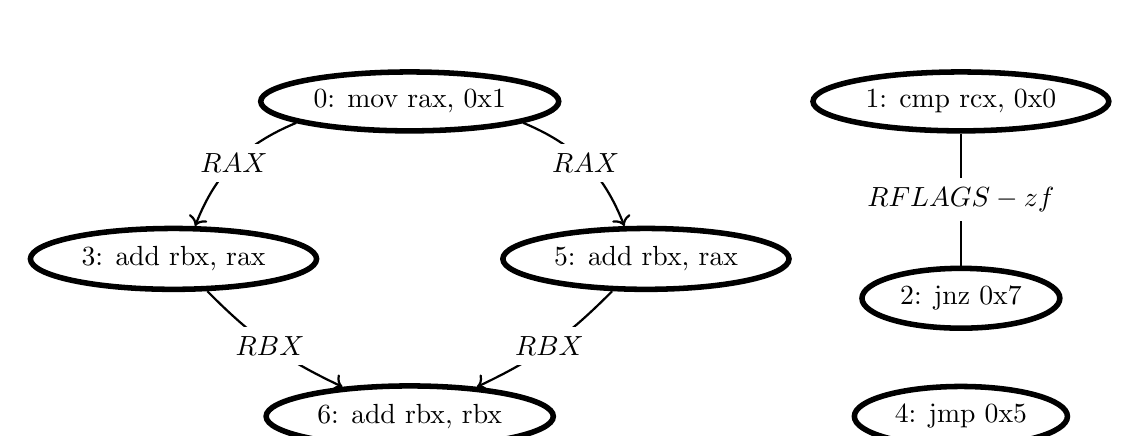
\begin{tikzpicture}
    \node[mynode] (A) at (-4, 0)  {0: mov rax, 0x1};	
    \node[mynode] (B) at (-7, -2) {3: add rbx, rax};
    \node[mynode] (C) at (-1, -2)  {5: add rbx, rax};
    \node[mynode] (D) at (-4, -4) {6: add rbx, rbx};


    \Edges[label=$RAX$, style=bright](A,B);
    \Edges[label=$RAX$, style=bleft](A,C);
    \Edges[label=$RBX$, style={->, bend right = 10}](B,D);
    \Edges[label=$RBX$, style={->, bend left = 10}](C,D);

    \node[mynode] (E)  at (3, 0)  {1: cmp rcx, 0x0};
    \node[mynode] (F)  at (3, -2.5) {2: jnz 0x7};
    
    \Edges[label=$RFLAGS - zf$](E,F);
    
    \node[mynode] (G)  at (3, -4) {4: jmp 0x5};

\end{tikzpicture}
\caption{Dependency graph without loop dependencies}
\label{fig:woloop}
\end{figure}


We can see that this graph was generated with the $CFG$ in mind as there is no edge from node $3$ to node $5$. Additionally we can observe that \suaca\ does differentiate between the different flags contained in the $RFLAGS$ register as the dependence is only reasoned with the $zf$ flag.\\
When \suaca\ is called with at least $2$ loops it will also track all ``loop dependencies''. \autoref{fig:wloop} shows the graph with those in consideration. We can see that two edges were added and they will be colored red to indicate that they were caused by the loops.

\begin{figure}
    \centering
    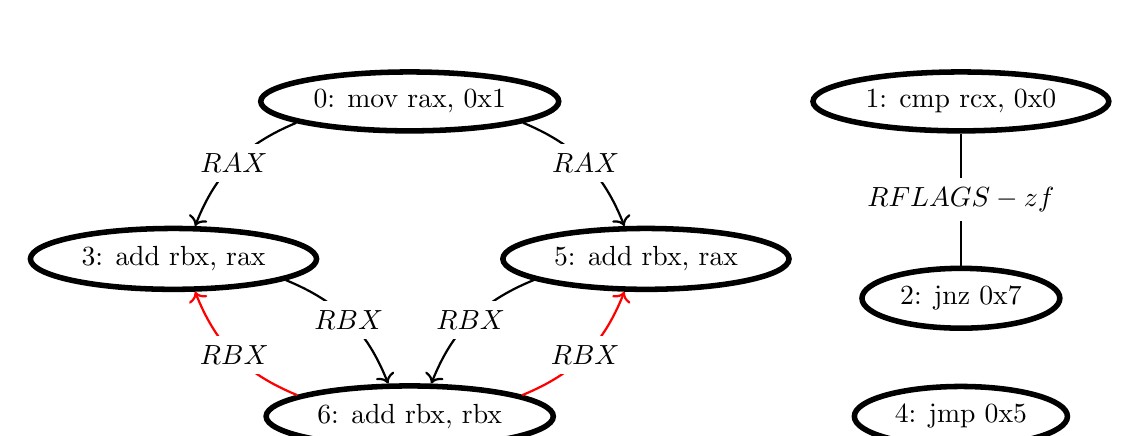
\begin{tikzpicture}
    \node[mynode] (A) at (-4, 0)  {0: mov rax, 0x1};	
    \node[mynode] (B) at (-7, -2) {3: add rbx, rax};
    \node[mynode] (C) at (-1, -2)  {5: add rbx, rax};
    \node[mynode] (D) at (-4, -4) {6: add rbx, rbx};
    
    
    \Edges[label=$RAX$, style=bright](A,B);
    \Edges[label=$RAX$, style=bleft](A,C);
    \Edges[label=$RBX$, style=bleft](B,D);
    \Edges[label=$RBX$, color = red, style=bleft](D, B);
    \Edges[label=$RBX$, style=bright](C,D);
    \Edges[label=$RBX$, color = red, style=bright](D, C);
    
    \node[mynode] (E)  at (3, 0)  {1: cmp rcx, 0x0};
    \node[mynode] (F)  at (3, -2.5) {2: jnz 0x7};
    
    \Edges[label=$RFLAGS - zf$](E,F);
    
    \node[mynode] (G)  at (3, -4) {4: jmp 0x5};
    
    \end{tikzpicture}
    \caption{Dependency graph with loop dependencies}
    \label{fig:wloop}
\end{figure}

\FloatBarrier

\section{Architecture selection}

As previously discussed one of the big a advantages of \suaca\ is that one can easily add new architectures that the analysis is based on.\\
The $--arch\ x$ option gives the user the ability to choose a specific micro-architecture. For our example we will use Intel's Coffee Lake micro-architecture instead of the Sandy Bridge micro-architecture we used previously (the first two columns are left out to improve readability):

\begin{mdframed}[backgroundcolor=light-gray, roundcorner=10pt,leftmargin=1, rightmargin=1, innerleftmargin=15, innertopmargin=15,innerbottommargin=15, outerlinewidth=1, linecolor=light-gray]
\begin{center}
\begin{BVerbatim}[fontsize=\tiny]
Block throughput: 2.00 cycles
Block throughput with perfect front end: 2.00 cycles
Block throughput with non-blocking ports: 2.00 cycles
Block throughput with perfect front end and non-blocking ports: 2.00 cycles
Microops per cycle: 3.49

Analysis for architecture: CFL

   had   || caused  ||            Used Ports
 to wait || to wait ||   0   ||   1   ||   2   ||   3   ||   4   ||   5   ||   6   ||   7   ||
------------------------------------------------------------------------------------------------------------
   4.7   ||  15.9   ||  0.1  ||  0.8  ||       ||       ||       ||  0.1  ||  0.1  ||       || mov rax, 0x1
   5.4   ||  13.6   ||  0.2  ||  0.5  ||       ||       ||       ||  0.1  ||  0.2  ||       || cmp rcx, 0x0
   6.2   ||   9.8   ||  0.4  ||       ||       ||       ||       ||       ||  0.6  ||       || jnz 0x7
  43.2   ||  48.9   ||  0.1  ||  0.2  ||       ||       ||       ||  0.7  ||  0.0  ||       || add rbx, rax
   5.1   ||   9.1   ||  0.2  ||       ||       ||       ||       ||       ||  0.8  ||       || jmp 0x5
  42.8   ||  51.6   ||  0.7  ||  0.1  ||       ||       ||       ||  0.2  ||  0.0  ||       || add rbx, rax
  43.6   ||  90.8   ||  0.1  ||  0.2  ||       ||       ||       ||  0.7  ||  0.0  ||       || add rbx, rbx
\end{BVerbatim}
\end{center}
\end{mdframed}

The most significant change is that the non-blocking ports analysis no longer experiences an improvement in runtime. This is due to the larger number of ports in the Coffee Lake architecture. We can now instead observe that the three $add$ instructions, or more so their dependencies on each other, are responsible for most of the delays.



\section{Detailed information}
\label{sec:detail}

\suaca\ can also deliver some detailed information about one particular line. This can be useful to determine how a specific instruction causes and experiences a delay. The following table shows the result of a run on our example program with $200$ iterations and details for line $0$.

\begin{mdframed}[backgroundcolor=light-gray, roundcorner=10pt,leftmargin=1, rightmargin=1, innerleftmargin=15, innertopmargin=15,innerbottommargin=15, outerlinewidth=1, linecolor=light-gray]
\begin{center}
\begin{BVerbatim}[fontsize=\scriptsize]
Detailed delay information for instruction: mov rax, 0x1 in line 0

                Maximum latency: 1
                
                Latencies for dependencies:
                
                Line || 0 -> Line || Line -> 0
                ----------------------------------
                 3   ||     1     ||     0
                 5   ||     1     ||     0
                
                
                Delay caused by dependencies:
                
                Line || was delayed || has delayed
                ----------------------------------
                 3   ||    15.2     ||     0.0
                 5   ||    14.5     ||     0.0
                
                
                Delay caused by blocked ports:
                
                Port || was delayed || has delayed
                ----------------------------------
                 0   ||     0.0     ||    15.1
                 1   ||    13.5     ||    15.1
                 5   ||     0.0     ||    15.1
\end{BVerbatim}
\end{center}
\end{mdframed}

In order to get a better understanding of those values we will split the output and explain them step by step.

\begin{mdframed}[backgroundcolor=light-gray, roundcorner=10pt,leftmargin=1, rightmargin=1, innerleftmargin=15, innertopmargin=15,innerbottommargin=15, outerlinewidth=1, linecolor=light-gray]
\begin{center}
\begin{BVerbatim}[fontsize=\scriptsize]
Maximum latency: 1

Latencies for dependencies:

Line || 0 -> Line || Line -> 0
----------------------------------
 3   ||     1     ||     0
 5   ||     1     ||     0
\end{BVerbatim}
\end{center}
\end{mdframed}

First we can see that this instruction has a maximum latency of one cycle. This value can differ from those of the table below as we have seen in ~\autoref{lst:xml}.\\
The table itself shows the latencies \suaca\ used for the dependencies. The second column show the delay from the analyzed line to the line given in the first column and the third row shows the delay in the other direction. In our case lines $3$ and $5$ depend on line $0$ (see ~\autoref{fig:wloop}) and we can see here that those lines actually have to wait one cycle for line $0$ to be finished and line $0$ itself is independent of the other two.\\

\begin{mdframed}[backgroundcolor=light-gray, roundcorner=10pt,leftmargin=1, rightmargin=1, innerleftmargin=15, innertopmargin=15,innerbottommargin=15, outerlinewidth=1, linecolor=light-gray]
\begin{center}
\begin{BVerbatim}[fontsize=\scriptsize]
Delay caused by blocked ports:

Port || was delayed || has delayed
----------------------------------
0   ||     0.0     ||    15.1
1   ||    13.5     ||    15.1
5   ||     0.0     ||    15.1
\end{BVerbatim}
\end{center}
\end{mdframed}

This table now shows, that lines $3$ and $5$ actually are delayed by our analyzed line. On average line $3$ has to wait $15.2$ cycles for line $0$ to be finished while line $5$ has to wait $14.5$ cycles. Of course both of them don't cause any delay on line $0$ as there is no dependence.\\

\begin{mdframed}[backgroundcolor=light-gray, roundcorner=10pt,leftmargin=1, rightmargin=1, innerleftmargin=15, innertopmargin=15,innerbottommargin=15, outerlinewidth=1, linecolor=light-gray]
\begin{center}
\begin{BVerbatim}[fontsize=\scriptsize]
Delay caused by blocked ports:

Port || was delayed || has delayed
----------------------------------
 0   ||     0.0     ||    15.1
 1   ||    13.5     ||    15.1
 5   ||     0.0     ||    15.1
\end{BVerbatim}
\end{center}
\end{mdframed}

Finally \suaca\ also tells you how much delay was caused by the ports. First consider that the $mov$ instruction in line $0$ can, in theory, use ports $0, 1$ and $5$. In our case it causes a delay of $13.5$ cycles per iteration on another instruction, because it uses port $1$. It doesn't cause any delay on the other two ports that it might use simply because it always uses port $1$ in our particular case (see ~\autoref{sec:loop}). The second column tells us that line $0$ experiences a delay of $15.1$ cycles per iteration because all three usable ports were blocked. The $mov$ instruction we're considering here only consists of a single \microop\ which leads to all three of those values being identical.\\
More precisely the $mov$ instruction can only be delayed by blocked ports if all three of its usable ports are blocked, otherwise it would just chose the free one. So all three of those blocked ports are responsible hence the three identical values.\\
However this is not always the case as an instruction might consist of more than one \microop. We will discuss this further in \autoref{sec:chooseport}.




\section{Branch analysis}

Finally \suaca\ is able to analyze different branches. As we have seen in \autoref{fig:cfg} and \autoref{fig:woloop} the ``normal'' analysis already considers branches for it's dependencies. However, as the effect of the instructions will be completely ignored in the simulation the branches won't have any other effect.\\
With the $-b$ flag one can trigger the actual branch analysis which will perform two simulations, one for each branch. This will always consider the first $jump$ instruction and this one only. It won't consider every single possible path through a program with multiple branches. This one $jump$ instruction, as well as the $jump$ instruction that's typically in one of the two branches, will be excluded from the analysis as \suaca\ expects the processor to perform branch prediction. We will now consider the branching analysis of our example program, again with the Sandy Bridge architecture and $200$ iterations:

\begin{mdframed}[backgroundcolor=light-gray, roundcorner=10pt,leftmargin=1, rightmargin=1, innerleftmargin=15, innertopmargin=15,innerbottommargin=15, outerlinewidth=1, linecolor=light-gray]
\begin{center}
\begin{BVerbatim}[fontsize=\tiny]
Left branch analysis:

Block throughput: 2.00 cycles
Block throughput with perfect front end: 2.00 cycles
Block throughput with non-blocking ports: 2.00 cycles
Block throughput with perfect front end and non-blocking ports: 2.00 cycles
Microops per cycle: 2.00

Analysis for architecture: SNB

Line  ||   Num   ||   had   || caused  ||            Used Ports
      ||   Uops  || to wait || to wait ||   0   ||   1   ||   2   ||   3   ||   4   ||   5   ||
------------------------------------------------------------------------------------------------
  0   ||    1    ||         ||   0.3   ||  0.5  ||  0.2  ||       ||       ||       ||  0.2  || mov rax, 0x1
  1   ||    1    ||         ||         ||  0.2  ||  0.5  ||       ||       ||       ||  0.3  || cmp rcx, 0x0
  3   ||    1    ||  45.4   ||  45.6   ||  0.3  ||  0.3  ||       ||       ||       ||  0.4  || add rbx, rax
  6   ||    1    ||  45.6   ||  45.4   ||  0.3  ||  0.3  ||       ||       ||       ||  0.4  || add rbx, rbx


Right branch analysis:

Block throughput: 2.00 cycles
Block throughput with perfect front end: 2.00 cycles
Block throughput with non-blocking ports: 2.00 cycles
Block throughput with perfect front end and non-blocking ports: 2.00 cycles
Microops per cycle: 2.00

Analysis for architecture: SNB

Line  ||   Num   ||   had   || caused  ||            Used Ports
      ||   Uops  || to wait || to wait ||   0   ||   1   ||   2   ||   3   ||   4   ||   5   ||
------------------------------------------------------------------------------------------------
  0   ||    1    ||         ||   0.3   ||  0.5  ||  0.2  ||       ||       ||       ||  0.2  || mov rax, 0x1
  1   ||    1    ||         ||         ||  0.2  ||  0.5  ||       ||       ||       ||  0.3  || cmp rcx, 0x0
  5   ||    1    ||  45.4   ||  45.6   ||  0.3  ||  0.3  ||       ||       ||       ||  0.4  || add rbx, rax
  6   ||    1    ||  45.6   ||  45.4   ||  0.3  ||  0.3  ||       ||       ||       ||  0.4  || add rbx, rbx
\end{BVerbatim}
\end{center}
\end{mdframed}

This kind of information can be useful to determine which of the two branches is more favorable for the execution. It can also be used to see if there are any significant differences between the two at all in order to prevent side channel attacks.\\
One can also use this in combination with the detailed analysis as \suaca\ will tell you the original line of all instructions in both parts of the branching analysis.

\section{Auxiliary}
The remaining options are:

\begin{itemize}
    \item $-p$ triggers the ``performance mode''. More specifically this will prevent the three extra analyses that are needed to generate the three additional block throughput values. In most cases however, \suaca's performance bottleneck will be the parser for the measurement files which cannot be deactivated. 
    \item ${--}setup\ x\ y$ sets the default values for the architecture ($x$) and the number of iterations ($y$). Note that one always has to use both values. 
    \item ${--}print-default$ prints the default values for architecture and number of iterations.
\end{itemize}









%----------------------------------------------------------------------------------------
%	Algorithms
%----------------------------------------------------------------------------------------

\chapter{Algorithms}
\label{chap:algorithms}

When trying to analyze a program the user sometimes needs to fully understand how the results were calculated. Especially if he wants use them to improve his code. Therefore we will discuss \suaca's most important algorithms in the following chapter.

\section{Dependency analysis}
\label{sec:depanalysis}

\subsection{Single iteration}

Here we want to take a look at the algorithm that computes the dependency graph. \\
First we want to discuss a simpler version that ignores the control flow of the program.

\begin{algorithm}[H]
    \SetAlgoLined
    \caption{Dependency analysis without control flow}
    \SetKwInOut{Input}{Input}
    \SetKwInOut{Output}{Output}
    \Input{Instructionlist InstList}
    \Output{Dependencygraph DG}
    Map $:=$ map from Register to line\;
    DG $:=$ Graph that has the same nodes as CFG, but no edges\;
    \ForEach{Instruction $i$ in InstList} {
         \ForEach{Register-Operand $r$ in Operands($i$)} {
             \eIf{IsRead($r$)} {
                 DG.addEdge(Map[$r$], LineOf($i$))\;
             }{
                Map[$r$] = LineOf(i)\;
            }
        }
    }
    \Return DG\;
\end{algorithm}

Where
\begin{itemize}
    \item $Operands(i)$ returns a list of all operands of instruction $i$.
    \item $IsRead(r)$ returns true if the operand $r$ will be read and false if it will be written to.
    \item $LineOf(i)$ returns the line of instruction $i$ in the original program.
\end{itemize}

This algorithm will iterate over all instructions ``line after line''. For each instruction $i$ it will then iterate over all of its operands. For each operand we'll check if it is accessed via read or write. If it is read the algorithm will add an edge from the last written access to the current line. If it is written to the algorithm will map the register to the current line.\\

The runtime of this algorithm can be described as $\mathcal{O}(n*m)$ where $n$ is the number of instructions and $m$ the maximum number of operands that occur in the program.\\

Note that we consider every operand as a register. In practice an operand can of course be a memory address. In this case \suaca\ will extract all registers from that address and treat them as a read operand. \suaca\ will not trace the memory itself.\\

Now we want to take a look at the control flow sensitive algorithm \suaca\ actually uses. 

\begin{algorithm}[H]
    \SetAlgoLined
    \caption{Control flow sensitive dependency analysis}
    \label{alg:dep}
    \SetKwFunction{deps}{Dep-Analysis-Start}
    \SetKwFunction{dep}{Dep-Analysis}
    \SetKwProg{Fn}{Function}{:}{\Return DG\;}
    \Fn{\deps{CFG}}{
        Map $:=$ map from Register to line\;
        DG $:=$ Graph that has the same nodes as CFG, but no edges\;
        Node $:=$ Startnode of CFG\;
        \dep{CFG, DG, Map, Node}\;
    }
    \SetKwProg{Fn}{Function}{:}{}
    \Fn{\dep{CFG, DG, Father-Map, Node}}{
        Map $:=$ copy of Father-Map\;
        \While{HasSuccessor(Node)} {
            \ForEach{Register-Operand $r$ in Operands($i$)} {
                \eIf{IsRead($r$)} {
                    DG.addEdge(Map[$r$], LineOf($i$))\;
                }{
                    Map[$r$] = LineOf(i)\;
                }
            }
            Node $\leftarrow$ Successor(Node, 0)\;
            \If{numSuccessors(Node) $>$ 1} {
                \dep{CFG, DG, Map, Successor(Node, 1)}\; 
            }
        }
    }
\end{algorithm}

Where
\begin{itemize}
    \item $numSuccessors(Node)$ returns the number of successors of $Node$ in its underlying graph.
    \item $Successor(Node, i)$ returns the $i$th successor of $Node$ in the Graph $Node$ belongs to.
    \item $HasSuccessor(Node)$ returns true if $numSuccessors(Node) >= 1$.
\end{itemize}

This time we'll ``climb along'' the $CFG$. If we never face a branch, i.e.\ $numSuccessors()$ never returns a value greater $1$, this algorithm will exactly the same as the one we have just seen.\\
In the case of $numSuccessors() > 1$ we'll make another call of $Dep-Analysis$ on the ``right branch''. From there on there will be $2$ analyses, one for every branch in the $CFG$. Each analysis has its own $Map$ as there can be different writes on each branch. Note that we won't join the two analyses as we would need to find the first mutual descendant.\\
In the worst case every instruction is a branch, so we would spawn a new function for every one of them. This leads to a runtime of $\mathcal{O}(n^2*m)$.\\
For this algorithm we assume no backbranches, i.e.\ no loops, inside the program. In practice \suaca\ will simply check for every branch if it is a backbranch and should the situation arise ignore it.


\subsection{Multiple iterations}

When telling \suaca\ to run the program in multiple loops we need to adjust the dependency analysis algorithm as there can arise some ``loop dependencies''. To solve this, we'll simply consider the program twice. So we'll append a copy of the program to itself, compute the $CFG$ and then run the algorithm above. Because we know the original length of our program we can extract all ``loop dependencies'' from the resulting dependency graph.


\section{Simulation the front end}
\label{sec:simfrontend}

Although our main task is to simulate the reservation station we still want to consider the front end in our analysis. Depending on the micro architecture the front end is able to produce a certain amount of \microops\ every cycle. For example the Sandy Bridge architecture will produce $4$ \microops\ per cycle. However, we still have to consider the capacity of the reservation station as the front end might be faster than the execution itself. The reservation station of the Sandy Bridge architecture has a maximum capacity of $54$ \microops.\\
We will now briefly discuss how our simulation actually performs those loads.

\begin{algorithm}[H]
    \SetAlgoLined
    \caption{Load instructions into reservation station}
    List $:=$ List of all instructions\;
    Waiting $:=$ First element of List that is not fully loaded\;
    Loadable $:= max(Loads\ per\ cycle, remaining\ space\ in\ station)$\;
    \While{Loadable $> 0$} {
        loaded $:=$ load\microops(Waiting, Loadable)\;
        Loadable $\leftarrow$ Loadable $-$ loaded\;
        \eIf{fullyLoaded(Waiting)} {
            Waiting $\leftarrow$ List.GetNextElement(Waiting)\;
        } {
            break\;
        }
    }
\end{algorithm}

Where
\begin{itemize}
    \item load\microops(Waiting, $x$) loads up to $x$ \microops\ of Waiting and returns the number of \microops\ that were actually loaded.
    \item $fullyLoaded(Waiting)$ returns true if all \microops\ of Waiting have been loaded into the reservation station.
    \item $List.GetNextElement(Waiting)$ returns the successor element of $Waiting$ in List.
\end{itemize}

So it is possible that an instruction is partially (i.e.\ only some of its \microops) loaded into the reservation station.

\section{Choosing the ports}
\label{sec:chooseport}

In this section we are going to discuss how exactly the ports which an instruction uses are chosen. As we've seen in \autoref{lst:xml} we know of how many \microops\ an instruction consists and which port those \microops\ want to use. As seen in \autoref{sec:simfrontend} an instruction can be loaded partially, which we will have to consider here.\\
The following algorithm contains several crucial details to the simulation. First we will see how \suaca\ tries to contribute all \microops\ equally over all ports. It will also demonstrate the exact situations in which we will execute an instruction. Lastly it will explain how the \textbf{had to wait} and \textbf{caused to wait} columns we introduced in \autoref{sec:plain} are computed. 

\begin{algorithm}[H]
    \SetAlgoLined
    \caption{Chose ports for loaded instructions}
    \SetKwInOut{Input}{Input}
    \Input{Instruction $:=$ First element in Instructionqueue}
    \While{loaded\_\microops(Instruction) $> 0$} {
        \eIf{$!all\_fathers\_done(Instruction)$} {
            Instruction.has\_to\_wait++\;
            \ForEach{Father $\in$ Fathers(Instruction)} {
                Father.caused\_to\_wait++\;
                Father.caused\_to\_wait\_depedency(Instruction)++\;
                Instruction.had\_to\_wait\_depedency(Father)++\;
            }
        } {
            Executable $:= true$\;
            \If{!is\_fully\_loaded(Instruction)}{Executable $\leftarrow false$\;}
            \ForEach{\microop\ $\mu$ $\in$ loaded\microops(Instruction)} {
                Success $:=$ assign\_to\_ports($\mu$, Instruction)\;
                \If{!Success} {
                    Executable $\leftarrow false$\;
                }
            }
            \eIf{Executable} {
                add\_to\_executionlist(Instruction)\; \label{line:if}
            }{
                Blamed $:=$ Set of instructions\; \label{line:else}
                \ForEach{p $\in$ blocked\_ports(Instruction)} {
                    \If{!Blamed.contains(p.using\_instruction())} {
                        p.using\_instruction().caused\_to\_wait++\;
                        p.using\_instruction().caused\_to\_wait\_port(p)\;
                        Instruction.had\_to\_wait\_port(p)\;
                        Blamed.add(p.using\_instruction())\;
                    }
                }
                Instruction.has\_to\_wait++\;
            }          
        }
        Instruction $\leftarrow$ Instructionqueue.next(Instruction)\;
    }
\end{algorithm}

~\\[-1em]
\begin{algorithm}[H]
    \label{alg:assign}
    \SetAlgoLined
    \caption{Assign \microop\ to port}
    \SetKwInOut{Input}{Input}
    \Input{\microop\ $\mu$, Instruction $I$}
    Success $\leftarrow true$\;
    \ForEach{p $\in$ PortQueue} {
        \If{$\mu$.can\_use(p) \textbf{and} p.is\_free()} {
            p.uses($\mu$)\;
            \Return $true$\;
        }
    }
    \Return Success\;
\end{algorithm}

So this algorithm iterates over all instructions in program order as long as the current instruction is at least partially loaded. For each instruction it will first check if all of its dependencies have been resolved. If not it can't be executed and the delay counters have to be increased. Notice that we have separate counters for the cumulative delays and the special delays, which are only needed for the detailed analysis (\autoref{sec:detail}). We will see the same behavior for the ports and this explains why the special delays won't always sum up to the cumulative ones.\\
If all dependencies have been resolved \suaca\ will try to assign all \microops\ of the instruction to a port. To achieve this the algorithm will iterate over all \microops\ that have been loaded into the reservation station. Note that this will ignore all \microops\ that have been put into a port already. The function \textbf{\emph{assign\_to\_ports(\microop, Instruction)}} is described in algorithm \ref{alg:assign}. This function will iterate over all ports in prior usage order and assign the \microop\ if possible. More precisely \emph{PortQueue} contains all ports and is sorted by usage throughout the whole simulation. If possible it will assign the \microop\ to the port and return a success. If no usable port was free it will return a fail. If all \microops\ of an instruction are currently in the port pipeline this algorithm will basically just put the instruction into the execution list.\\
We can observe that this is a greedy algorithm that is obviously not optimal in regards to the distribution of all \microops\ over the ports. However, we assume that this greedy algorithm comes close to what the reservation stations are doing in reality.\\
If the assignment or the load of a single \microop\ failed the flag \emph{Executable} will be set to \emph{false}. As we can see in \autoref{line:if} the instruction will only added to the execution list (which we will further discuss in \autoref{sec:execute}) if this flag is set. This means that an instruction is only executed if all of its \microops\ could be assigned to a port. We are doing this, because of our measurements. As we've seen in \autoref{sec:measurements} those will always contain the best case for latency. The biggest problem we face here is the missing information about the \microops. We don't know anything about the dependencies between them and so we don't know if there is an order in which those have to be executed, or if they can be executed simultaneously. So we have to assume a delay as soon as a single \microop\ is denied a port although that might not actually be the case in reality. This means that we will potentially overestimate the latency of a single instruction although it is possible that \suaca\ will actually underestimate the throughput of a program as one can note in the following examples.\\


Consider two instructions \emph{X} and \emph{Y}. \emph{X} consists of two \microops\ one of which can use port $0$ the other can use port $1$. \emph{Y} only consists of one which can use port $1$. \emph{X} is in front of \emph{Y} in program order, both are fully loaded, not dependent on each other and have a latency of $2$ cycles.\\
What \suaca\ ``doesn't know'' is that the the second \microop\ (port $1$) of \emph{X} depends on the first (port $0$). So the simulation will do the following: In the first cycle it will assign \emph{X} to ports $0$ and $1$. There is no port left for \emph{Y} so it won't be added to the execution list. This will happen in the second cycle and as \emph{Y}'s latency was two cycles \suaca\ will compute a throughput of three cycles (as \emph{X} was executed in the first and second).\\
However, in reality \emph{X} won't block port $1$ in the first cycle as this particular \microop\ depends on the one that uses port $0$. So in the first cycle \emph{X} will only use port $0$. \emph{Y} can then freely use port $1$. In the second cycle \emph{X} can then use port $1$. No port was ever blocked so there simply won't be a delay, both instructions could be executed simultaneously. So the ``real throughput'' of our example would be two cycles.\\

Now we will consider the same example but with switched instruction order of \emph{X} and \emph{Y}. In this case \suaca\ will first assign \emph{Y}'s \microop\ to port $1$. It will then try to assign \emph{X}, but it will only be able to assign the first \microop\ to port $0$ as port $1$ is blocked. As discussed before \emph{X} will therefore not be added to the execution list. In the second cycle the leftover of \emph{X} will be assigned to a port and the execution will start. As the latency was two cycles the simulation will stop after the third cycle.\\
Again this is an overestimation of the reality. Due to the dependency of the second \microop\ of \emph{X} it doesn't matter that \emph{Y} blocks port $1$ in the first cycle. \emph{X} only needs port $0$ in the first cycle and in the second cycle it can then freely use port $1$. Again the ``real throughput'' of our example would be two cycles.\\

Finally we will construct an example were our simulation actually underestimates the throughput. We can once more use our two instructions \emph{X} and \emph{Y}. This time we assume that \emph{Y} can't be executed in the first cycle, because of a dependency. Our simulation basically works like in our first case, except for the reason why \emph{Y} can't be executed. So it will compute a throughput of three cycles for those two instructions.\\
In reality \emph{Y} will be denied port $1$ in the second cycle as it will by used by \emph{X}. So the execution will start in the third cycle and end in the fourth.\\

Note that it is still impossible that the latency of a single instruction is underestimated as we will always simulation the execution of at least as many cycles as we measured under a best case scenario.\\

Ultimately we will consider the rest of the algorithm starting in \autoref{line:else}. This part will increase the counters similar to what we've seen at the start of the algorithm. Notable here is the function \textbf{\emph{blocked\_ports(Instruction)}} that will return all ports that have been blocked during the assignment phase.

%TODO explain groups of microops


\section{Executing applicable instructions}
\label{sec:execute}

\begin{algorithm}[H]
    \SetAlgoLined
    \caption{Execute applicable instructions}
    \ForEach{I $\in$ Executionlist} {
        I.executed\_cycles$++$\;
        \If{I.executed\_cycles $=$ I.latency} {
            Instructionqueue.remove(I)\;
        }
        inform\_children\_im\_done(I)\;
    }
    Executionlist.clear()\;
\end{algorithm}

This part is rather simple. Every instruction knows its latency and how many cycles it has been executed. This value gets increased and if the latency is hit it will be removed from the Instructionqueue. The most interesting part here is the function \textbf{\emph{inform\_children\_im\_done(Instruction)}}. As we've seen in \autoref{sec:measurements} the children of an instruction don't necessarily have to wait for the instruction to finish. Sometimes they only need part of the results, which are available earlier. So this function will iterate over all children and check if the execution is advanced enough and if so ``release the dependency''. Finally we have to clear the execution list as we will fill it again in the next cycle.

\section{Performing a cycle}

Lastly we want to briefly discuss how a whole cycle is performed. \suaca\ will run each of the three simulation algorithms we explained above. It will then free up all ports, that were used during the cycle, in order to enable the port pipelining. A short pseudo code representation can be found below.

\begin{algorithm}[H]
    \SetAlgoLined
    \caption{Perform a whole cycle}
    load\_instructions()\;
    choose\_ports()\;
    execute\_instructions()\;
    \ForEach{p $\in$ Ports} {
        p.clear()\;
    }
\end{algorithm}

The interesting observation here is that an instruction can actually get loaded, put into a port and then executed within a single cycle, due to the order of the function calls.

\chapter{Evaluation}

%\bibliographystyle{ieeetr}
%{\small \bibliography{cites}}
\printbibliography


\end{document}
